
\title{T-61.5130 Machine Learning and Neural Networks}
\author{Karhunen, Luttinen}
\date{Exercise 8}

\newcommand{\vect}[1]{{\bf{#1}}}
\newcommand{\svect}[1]{\boldsymbol{#1}}
\newcommand{\matr}[1]{\boldsymbol{#1}}

\renewcommand{\vec}[1]{\mathbf{#1}}
\newcommand{\set}[1]{\mathcal{#1}}
\newcommand{\C}{\set{C}}
\newcommand{\E}{\mathcal{E}}
\newcommand{\I}{\vec{I}}
\renewcommand{\L}{\mathcal{L}}
\newcommand{\N}{\mathrm{I \negmedspace N}}
\newcommand{\R}{\mathrm{I \negmedspace R}}
\newcommand{\V}{\set{V}}
\newcommand{\W}{\vec{W}}
\newcommand{\X}{\set{X}}
\newcommand{\e}{\vec{e}}
% \newcommand{\f}[1]{\mathrm{#1}} %funktio
\newcommand{\h}{\vec{h}}
\newcommand{\m}{\vec{m}}
\newcommand{\mub}{\boldsymbol{\mu}}
\newcommand{\n}{\vec{n}}
\renewcommand{\t}{\vec{t}}
\renewcommand{\u}{\vec{u}}
\renewcommand{\v}{\vec{v}}
\newcommand{\w}{\vec{w}}
\newcommand{\x}{\vec{x}}
\newcommand{\y}{\vec{y}}
\newcommand{\Y}{\vec{Y}}
\newcommand{\z}{\vec{z}}
\newcommand{\argmin}{\operatornamewithlimits{argmin}}
\newcommand{\argmax}{\operatornamewithlimits{argmax}}


\begin{document}

\maketitle
\thispagestyle{empty}

\begin{enumerate}

\item Starting with the primal problem for the optimization of the
  separating SVM-hyperplane for nonseparable patterns, formulate the
  dual problem for the nonseparable case.

  \begin{solution}

    First, consider a general constrained optimization problem:
    \begin{align*}
      \text{minimize}& \quad f(x)
      \\
      \text{subject to}& \quad g(x) \leq 0.
    \end{align*}
    If a point $x$ is an optimum and $g(x)\leq 0$, the point needs to
    satisfy:
    \begin{align*}
      \text{if } g(x)<0:& \quad \nabla f(x) = 0
      \\
      \text{if } g(x)=0:& \quad \nabla f(x) = -\alpha \nabla g(x),
      \quad \text{where } \alpha \geq 0.
    \end{align*}
    Therefore, we have the following conditions:
    \begin{align*}
      \nabla f(x) + \alpha \nabla g(x) = 0
      \\
      \alpha g(x) = 0
      \\
      g(x) \leq 0
      \\
      \alpha \geq 0,
    \end{align*}
    where the second condition means that either $\alpha$ or $g(x)$
    must equal to zero.  These conditions are equal to optimizing the
    following Lagrangian function:
    \begin{align*}
      & \quad \min_x \max_\alpha f(x) + \alpha g(x)
      \\
      \text{subject to} &\quad g(x) \leq 0
      \\
      &\quad \alpha \geq 0.
    \end{align*}
    By solving $x$ from $\nabla f(x) + \alpha \nabla g(x) = 0$ and
    inserting it to the Lagrangian cost function, one obtains the dual
    form.

    Now, let us examine our SVM problem.  We want to maximize the
    separation:
    \begin{align*}
      \max \frac{2}{\|\mathbf{w}\|} \Rightarrow \min \|\mathbf{w}\|
      \Rightarrow \min \|\mathbf{w}\|^2 \Rightarrow \min
      \frac{1}{2} \mathbf{w}^T\mathbf{w}.
    \end{align*}
    For a linearly separable problem we have:
    \begin{align*}
      d_i(\mathbf{w}^T\mathbf{x}_i + b) \geq 1, \quad \text{where }
      d_i =
      \begin{cases}
        +1, \quad \text{if } \mathbf{x}_i \text{ in class 1}
        \\
        -1, \quad \text{if } \mathbf{x}_i \text{ in class 2}
      \end{cases}
    \end{align*}
    In order to handle a linearly non-separable problem, we add slack
    variables $\xi_i$:
    \begin{align*}
      d_i(\mathbf{w}^T\mathbf{x}_i + b) \geq 1 - \xi_i, \quad
      \text{where } \xi_i \geq 0 \text{ and } d_i =
      \begin{cases}
        +1, \quad \text{if } \mathbf{x}_i \text{ in class 1}
        \\
        -1, \quad \text{if } \mathbf{x}_i \text{ in class 2}
      \end{cases}
    \end{align*}
    In addition to maximizing the separation, we want to minimize the
    classification errors, that is, minimize the slack variables
    $\xi_i$.  Thus, the optimization problem is now:
    \begin{align*}
      \text{minimize} &\quad \frac{1}{2} \mathbf{w}^T\mathbf{w} + C
      \sum_i \xi_i
      \\
      \text{subject to} &\quad d_i(\mathbf{w}^T\mathbf{x}_i + b) \geq
      1 - \xi_i,
      \\
      &\quad
      \xi_i \geq 0,
    \end{align*}
    where $C$ is a trade-off parameter between the separation and the
    classification errors.  Now the Lagrangian function is
    \begin{align*}
      J(\w, b, \xi, \alpha, \beta) = \frac{1}{2}\w^T\w + C
      \sum_{i=1}^N \xi_i - \sum_{i=1}^N \alpha_i[d_i(\w^T \x_i + b) -
      1 + \xi_i] - \sum_{i=1}^N \beta_i \xi_i
    \end{align*}
    where $\alpha_i$ and $\beta_i$ are Lagrange multipliers.  The
    conditions for optimality are $\partial J/\partial \w = \vec{0}$,
    $\partial J/\partial b = 0$ and $\partial J/\partial \xi =
    \vec{0}$.  We thus have
    \begin{align*}
      &\frac{\partial J}{\partial \w} = \w - \sum_{i=1}^N \alpha_i d_i
      \x_i = 0 \; \Rightarrow \; \w = \sum_{i=1}^N \alpha_i d_i \x_i
      \, ,
      \\
      &\frac{\partial J}{\partial b} = - \sum_{i=1}^N \alpha_i d_i = 0
      \,
      \\
      &\frac{\partial J}{\partial \xi_i} = C - \alpha_i - \beta_i = 0
      \; \Rightarrow \; \alpha_i + \beta_i = C \, .
    \end{align*}
    Inserting these to the Lagrangian function gives after some
    manipulation
    \begin{align*}
      &\quad J(\w, b, \xi, \alpha, \beta)
      \\
      &= \frac{1}{2}\w^T\w + C \sum_{i=1}^N \xi_i - \sum_{i=1}^N
      \alpha_i[d_i(\w^T \x_i + b) - 1 + \xi_i] - \sum_{i=1}^N \beta_i
      \xi_i
      \\
      &= \underbrace{\frac{1}{2}\w^T\w - \w^T \sum_{i=1}^N \alpha_i
        d_i \x_i}_{=-\frac{1}{2}\w^T\w} +
      \sum_{i=1}^N\underbrace{(C-\alpha_i-\beta_i)}_{=0}\xi_i - b
      \underbrace{\sum_{i=1}^N\alpha_i d_i}_{=0} + \sum_{i=1}^N
      \alpha_i
      \\
      &= \sum_{i=1}^N \alpha_i - \frac{1}{2} \sum_{i=1}^N
      \sum_{j=1}^N \alpha_i \alpha_j d_i d_j \x_i^T \x_j
      \\
      &= Q(\alpha)
    \end{align*}
    This is the objective function of the dual problem.  In addition
    to the constraint $\alpha_i\geq 0$, we have derived some constraints from
    the optimality conditions.  Thus, the dual problem is
    \begin{align*}
      \text{maximize} &\quad \sum_{i=1}^N \alpha_i - \frac{1}{2} \sum_{i=1}^N
      \sum_{j=1}^N \alpha_i \alpha_j d_i d_j \x_i^T \x_j
      \\
      \text{subject to} &\quad 0 \leq \alpha_i \leq C
      \\
      &\quad \sum_{i=1}^N \alpha_i d_i = 0,
    \end{align*}
    where $\alpha_i \leq C$ follows from the constraints $\alpha_i +
    \beta_i = C$ and $\beta_i \geq 0$.  The constraint $\alpha_i \leq
    C$ is also the only difference to the dual problem of the linearly
    separable problem without slack variables.  If $C$ is small, the
    data is assumed to be noisy.  After the optimal $\alpha_i$ are
    found, the SVM parameters $\mathbf{w}$ and $b$ can be computed.

    The dual problem has the following nice properties:
    \begin{itemize}
    \item The optimization problem is cast entirely in terms of the
      training data.
    \item $Q(\alpha)$ depends on the input patterns only in the form
      of a set of dot products $\x_i^T\x_j$.  Thus, the input
      variables can be transformed non-linearly with a kernel trick by
      changing $\x_i^T\x_j$ to $k(\x_i,\x_j)$.
    \end{itemize}
    

    % $$Q(\alpha) = \sum_{i=1}^N \alpha_i - \frac{1}{2} \sum_{i=1}^N
    % \sum_{j=1}^N \alpha_i \alpha_j d_i d_j \x_i^T \x_j \, ,$$ where
    % $Q(\alpha) = J(\w, b, \xi, \alpha, \mu)$ is the objective function
    % of the dual problem.

    % See also exercise 5 in T-61.5130 (pattern recognition) available
    % in Noppa, which contains more derivations.
  \end{solution}
  
\item In the case of separable classes, what happens to the separating
  hyperplane of SVMs if the amount of noise increases? How about the
  case of nonseparable classes?

  \begin{solution}

    The separating hyperplane is determined by the samples which are
    closest to the wrong class.  With no noise the hyperplane will be
    optimal in the sense that the margin of separation will be as wide
    as possible.  With increasing noise the orientation of the
    hyperplane changes randomly because the positions of the support
    vectors change.  At some point when the noise has increased enough,
    the samples have moved to points which cannot be linearly separated.
    Then the separation can be done using slack-variables which allow
    some points to be on the wrong side of the separating hyperplane.
    Notice that the number of support vectors does not change.

    % "The number of support vectors does not change." ???
    %
    % That claim needs a bit of a proof!!!
    
  \end{solution}
  
\item The inner-product kernel for a polynomial learning machine is
  defined by
  \begin{displaymath}
    k(\x,\x_i) = (1 + \x^T \x_i)^p \; ,
  \end{displaymath}
  where $p$ is a positive integer.  What is the dimension of the
  implicit feature space if the dimension of $\x$ is $m$.  Find lower
  and upper bounds if you cannot find the exact answer.

  \begin{solution}

    Any inner-product kernel can be represented as
    \begin{align*}
      k(\x_i,\x_j) &= \sum_{d=1}^D \phi_d(\x_i) \phi_d(\x_j)
      \\
      &= \boldsymbol{\phi}(\x_i)^T \boldsymbol{\phi}(\x_j)
    \end{align*}
    where $D$ is the dimensionality of the implicit feature space and
    $\phi_d$ are non-linear transformations to the feature space.  In
    general, the dimensionality $D$ can be infinite.

    Now, our inner-product kernel is $K(\x, \y) = (1 + x_1 y_1 +
    \ldots x_m y_m)^p$.  For instance, $m=2$ and $p=2$ yields
    \begin{align*}
      k(x, y) &= (1 + x_1y_1 + x_2y_2)^2
      \\
      &= 1 + 2x_1y_1 + 2x_2y_2 + x_1^2y_1^2 + x_2^2y_2^2 +
      2x_1x_2y_1y_2
      \\
      &=
      \begin{bmatrix}
        1 & \sqrt{2}x_1 & \sqrt{2}x_2 & x_1^2 & x_2^2 & \sqrt{2}x_1
        x_2
      \end{bmatrix}
      \begin{bmatrix}
        1 & \sqrt{2}y_1 & \sqrt{2}y_2 & y_1^2 & y_2^2 & \sqrt{2}y_1
        y_2
      \end{bmatrix}^T .
    \end{align*}
    Therefore the implicit features are $1$, $\sqrt{2}x_1$,
    $\sqrt{2}x_2$, $x_1^2$, $x_2^2$ and $\sqrt{2}x_1 x_2$, i.e., the
    dimension of the implicit feature space is six.

    In general, each term of $k(\x, \y)$ is of the form
    \begin{align*}
      c 1^{p_0} x_1^{p_1} y_1^{p_1} \ldots x_m^{p_m} y_m^{p_m} =
      (\sqrt{c} x_1^{p_1} \ldots x_m^{p_m})(\sqrt{c} y_1^{p_1} \ldots
      y_m^{p_m}),
    \end{align*}
    where c is an integer and $\sum_{i=0}^m p_i = p$.  This shows that
    the implicit features are of the form $\sqrt{c} x_1^{p_1} \ldots
    x_m^{p_m}$ and the dimension of the implicit feature space is the
    number of these terms, i.e., the number of partitions $p_i$ which
    satisfy $\sum_{i=0}^m p_i = p$.

    In order to evaluate the number of partitions, we shall construct a
    scheme for coding the numbers $p_i$ as a sequence.  For each $i$,
    the sequence contains $p_i$ symbols $a$ and the border between
    different $p_i$ is denoted by delimiter $b$.  Since there are $m+1$
    numbers $p_i$, the sequence has $m$ symbols $b$.  It is easy to see
    that each sequence having $p$ symbols $a$ and $m$ symbols $b$ can be
    interpreted as a unique set of numbers $p_i$ and vice versa.The
    number of these sequences and therefore also the dimension of the
    implicit feature space is
    \begin{align*}
      \frac{(m+p)!}{m!p!}.
    \end{align*}
    (The sequence has length $m+p$ but there are $p$ exchangeable
    symbols $a$ and $m$ exchangeable symbols $b$.)
    
    In short, one can use the formula for the number of combinations
    with repetition.  Now we have $m+1$ elements and $p$-combinations:
    \begin{align*}
      D = \binom{m+1+p-1}{p} = \binom{m+p}{p} =
      \frac{(m+p)!}{p!(m+p-p)!}  = \frac{(m+p)!}{m!p!}.
    \end{align*}
  \end{solution}
  

\item Can a support vector machine be used to solve a pattern
  classification task where there are more than two classes?

  \begin{solution}

    Yes.  For each class, construct a SVM which discriminates
    between that class and all the rest.  This way there will be as many
    SVMs as there are classes.  Alternatively, it is possible to use a
    binary classification as the following example shows: for eight
    classes, train one SVM to separate between classes (1,2,3,4) and
    (5,6,7,8), one SVM to separate between (1,2,5,6) and (3,4,7,8) and
    one SVM to separate (1,3,5,7) and (2,4,6,8).  This way there will be
    only about $\log_2 N$ classifiers for $N$ classes, but the task for
    each SVM will be more difficult and consequently the classification
    result can be worse.

  \end{solution}


\item (demo) Solve the double-moon classification problem with SVM.

  \begin{solution}
    The following figures are from Simon Haykin \emph{Neural Networks
      and Learning Machines (Third Edition)} 2009 (Pearson Education).

    \begin{center}
      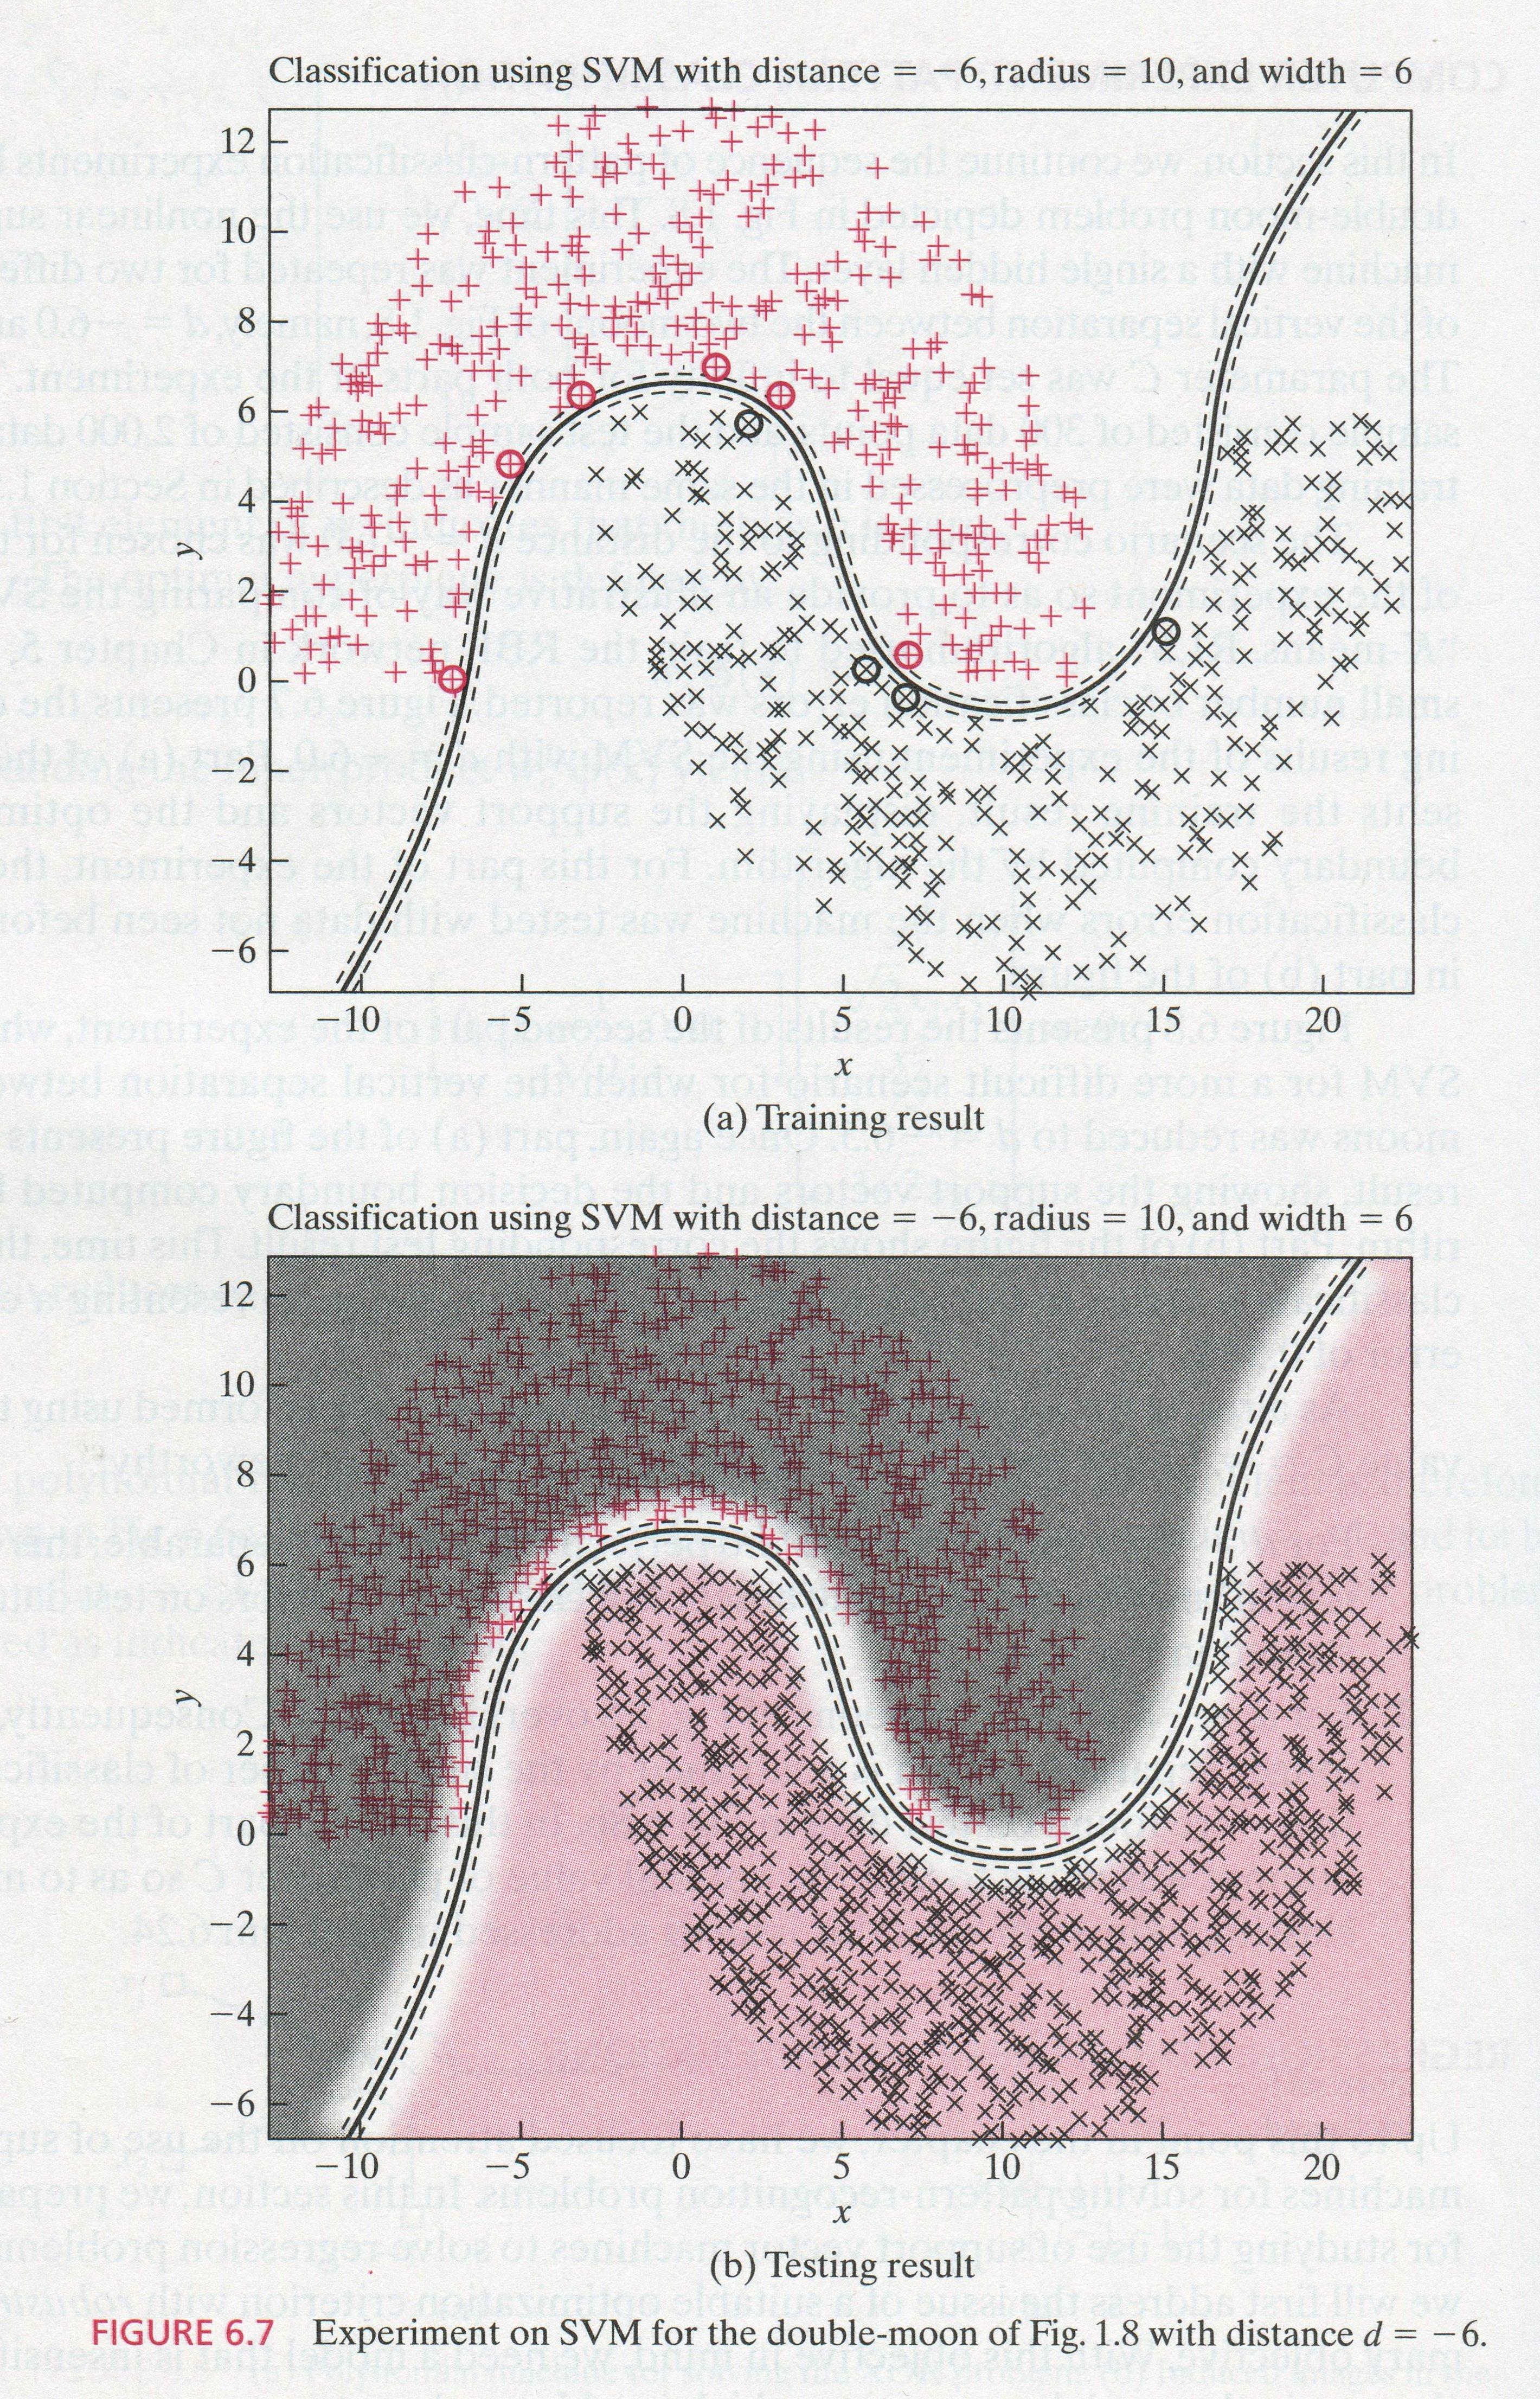
\includegraphics[width=0.7\linewidth]{ex08_05_svm.jpg}
    \end{center}
  \end{solution}
    
\end{enumerate}
\end{document}             % End of document.

%%% Local Variables: 
%%% mode: latex
%%% TeX-master: "ex08_solutions"
%%% End: 
